% Supply Projection Graph
% Shows circulating supply growth over 20 years
%
% ACCESSIBILITY ALT TEXT:
% A line graph showing total BTH supply over 20 years. X-axis shows years,
% Y-axis shows total supply in millions of BTH. The curve rises steeply
% initially as block rewards are high, then gradually flattens as rewards
% decay toward tail emission. Asymptotic supply approaches approximately
% 100 million BTH. A secondary annotation shows inflation rate declining
% from initial double digits to approximately 2% during tail emission phase.

\begin{figure}[ht]
\centering
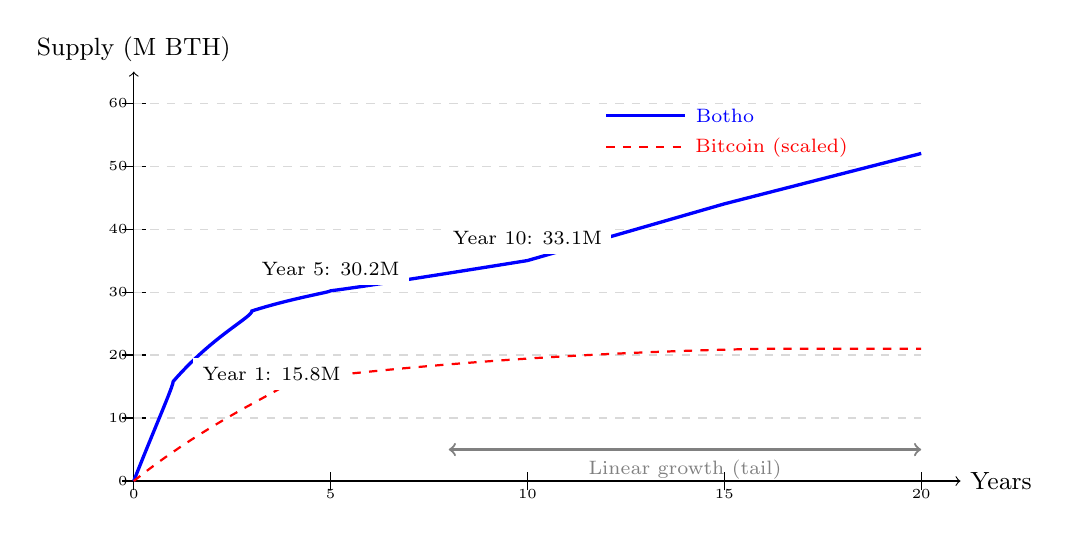
\begin{tikzpicture}[xscale=0.5, yscale=0.08]
    % Axes
    \draw[->] (0,0) -- (21,0) node[right] {\small Years};
    \draw[->] (0,0) -- (0,65) node[above] {\small Supply (M BTH)};

    % Y-axis labels
    \foreach \y in {0,10,20,30,40,50,60} {
        \draw (-0.3,\y) -- (0.3,\y) node[left=3pt] {\tiny \y};
    }

    % X-axis labels
    \foreach \x in {0,5,10,15,20} {
        \draw (\x,-1.5) -- (\x,1.5) node[below=3pt] {\tiny \x};
    }

    % Grid
    \foreach \y in {10,20,30,40,50,60} {
        \draw[gray!30, dashed] (0,\y) -- (20,\y);
    }

    % Botho supply curve (approximation)
    % Rapid initial growth, then linear tail emission
    \draw[blue, very thick]
        (0,0)
        .. controls (0.5,8) and (1,15) .. (1,15.8)
        .. controls (2,23) and (3,26) .. (3,27)
        .. controls (4,29) and (5,30) .. (5,30.2)
        .. controls (6,31) and (8,33) .. (10,35)
        -- (15,44)
        -- (20,52);

    % Bitcoin comparison (scaled, capped at 21)
    \draw[red, thick, dashed]
        (0,0)
        .. controls (2,10) and (4,15) .. (4,16)
        .. controls (8,19) and (12,20.5) .. (16,21)
        -- (20,21);

    % Key milestones
    \node[anchor=west, font=\scriptsize, fill=white] at (1.5,17) {Year 1: 15.8M};
    \node[anchor=south, font=\scriptsize, fill=white] at (5,31) {Year 5: 30.2M};
    \node[anchor=south, font=\scriptsize, fill=white] at (10,36) {Year 10: 33.1M};

    % Legend
    \draw[blue, very thick] (12,58) -- (14,58) node[right, font=\scriptsize] {Botho};
    \draw[red, thick, dashed] (12,53) -- (14,53) node[right, font=\scriptsize] {Bitcoin (scaled)};

    % Tail emission annotation
    \draw[<->, gray, thick] (8,5) -- (20,5) node[midway, below, font=\scriptsize] {Linear growth (tail)};
\end{tikzpicture}
\caption{Projected circulating supply over 20 years. Initial emission follows
exponential decay (similar to Bitcoin's halving schedule but smooth),
transitioning to linear growth from perpetual tail emission after approximately
year 6. Unlike Bitcoin's hard cap at 21M, Botho's supply grows indefinitely
at a declining percentage rate, ensuring permanent security funding.}
\label{fig:supply-projection}
\end{figure}
